% What makes a genomic language model memorise?  --  RECOMB 2027 submission.
%
% RULES TAKEN FROM THE 2027 CALL (recomb.org/recomb2027/call_for_papers, read 9 Oct 2026):
%   * abstract due 28 Oct 2026 23:59 AoE, full paper 4 Nov 2026, notification 22 Dec 2026,
%     conference 17-20 May 2027.
%   * 10 pages maximum, Letter, INCLUDING all figures, tables and captions; bibliography excluded.
%   * minimum 10pt font and 1-inch margins; PDF; no required template (LNCS optional).
%   * one extra title page with title, authors and abstract is allowed and does not count.
%   * single-blind: do NOT anonymise.
%   * optional appendix as a SEPARATE PDF with no page limit -> appendix.tex, built on its own.
%   * a paper with new software must link a public, documented repository IN the paper.
%   * at most 4 submissions per author; the registered abstract must match the final paper.
%   * accepted papers must be posted to bioRxiv/arXiv by the final-version deadline.
%
% PAGE BUDGET for the 10 content pages, privacy-first (notes/21_privacy_first_plan.md):
%   1 intro                        1.00    5 identification (1 table)     1.50
%   2 background + related         0.75    6 slot count (1 table, 1 fig)  1.50
%   3 threat model + measurement   1.25    7 practice + blind metric      1.25
%   4 leak at usable quality       1.75    8 limitations + discussion     0.75
%   slack 0.25. Five figures is already 1.25-1.5 of the ten; F1 (probe geometry) is the
%   first to cut, and fig:slots is load-bearing and may not move to the appendix.
%
\documentclass[10pt,letterpaper]{article}
\usepackage[margin=1in]{geometry}

\usepackage[T1]{fontenc}
\usepackage[utf8]{inputenc}
\usepackage{times}
\usepackage{graphicx}
\usepackage{booktabs}
\usepackage{multirow}          % tab:objaxis pairs two objective rows per dataset
\usepackage{amsmath,amssymb}
\usepackage{siunitx}
\usepackage{microtype}
\usepackage{xcolor}
\usepackage[hidelinks]{hyperref}
\usepackage{subcaption}
\usepackage[font=small,labelfont=bf]{caption}
\usepackage{authblk}

\graphicspath{{figures/}}
\sisetup{detect-all, group-minimum-digits=4}
\renewcommand{\arraystretch}{1.05}

% ---------------------------------------------------------------- shared macros
\newcommand{\bits}{bits/nt}                       % every score is per nucleotide
\newcommand{\nt}{\,nt}
\newcommand{\kmer}[1]{#1-mer}
\newcommand{\excess}{\ensuremath{\Delta}}         % non-member bits minus member bits
\newcommand{\TODO}[1]{\textcolor{red}{[TODO: #1]}}
\newcommand{\NUM}[1]{\textcolor{blue}{#1}}        % number still pending a run; must be black at submission
\newcommand{\CODEURL}{\TODO{public repository URL -- required by the call}}

\title{\textbf{Released Genomic Language Models Identify the People\\They Were Fine-Tuned On}\\[2pt]
\large Reproduction Is the Wrong Alarm, and Tokenisation Explains Why}
\author[1]{Yiqian Zhang}
\author[1]{Alexander Nemecek}
\author[1]{\TODO{co-authors and order to be agreed}}
\author[1]{Erman Ayday}
\affil[1]{Department of Computer and Data Sciences, Case Western Reserve University, Cleveland, OH, USA}
\date{}

\begin{document}

% ---- extra title page (allowed by the call, does not count against the 10 pages)
\begin{titlepage}
\maketitle
\thispagestyle{empty}
\begin{abstract}
% ~215 words. The claim ladder in the order the paper makes it. Must match the registered
% abstract, so change this and the contribution list of p01_intro together.
Genomic language models are released pretrained and fine-tuned locally, increasingly on cohort data.
We ask what happens to the individuals in that cohort, and measure it on six released models rather
than on a backbone of our own.

Every released masked checkpoint we tested reproduces planted records verbatim at a held-out loss a
practitioner would accept: the cheapest costs seven thousandths of a bit and returns 30\% of records.
On real chromosome-22 haplotypes, each carried by at most five of 2{,}548 individuals, a record
present as a single copy comes back letter for letter about one time in ten.

Reproduction is the wrong alarm. At checkpoints where verbatim recovery reads exactly zero in every
seed, the same model ranks one individual's haplotype first against a hundred real rare segments
0.92 to 0.96 of the time, with none of 350 never-trained controls ever identified. Downstream task
score moves one to two per cent across the same range.

Whether a memorised record can be reached at all is set by how many token slots it occupies, not by
how much the model knows: models differing only in tokenisation answer any single hidden nucleotide
identically and yet return 92\% or 0\% of whole records. No single extraction test is correct across
tokenizers, which is why this has been missed. Code, measurements and logs are public.

\end{abstract}
\vfill
\noindent\textbf{Code and data.} \CODEURL. All inputs are public: 1000~Genomes phase~3 (chr22,
GRCh38), the GUE benchmark, and the reference genomes of \emph{E.~coli} K-12 MG1655 and
\emph{S.~cerevisiae} S288C.
\end{titlepage}

\setcounter{page}{1}

% Privacy-first structure, settled 19 Oct: the privacy results lead and the tokenisation and
% measurement work supports them. The objective-first draft is kept in main_objective_first.tex.bak
% and sections/0*_*.tex until this one is checked end to end.
% Privacy-first section 1. Budget 1.0 page, no figure.
\section{Introduction}
\label{sec:intro}

Genomic language models are released pretrained and fine-tuned locally, increasingly on cohort data
that the releasing laboratory never sees. A group with a few thousand participants' sequences adapts
a published checkpoint, reports a downstream metric, and shares the weights. We ask what that
sharing does to the people in the cohort.

A recent study established that published genomic models memorise their fine-tuning sequences to
very different degrees, without identifying what causes the difference
\citep{nemecek2026quantifying}. The natural follow-up is to find the cause, and we do; but the more
consequential finding turned out to be that the safety check the field applies to answer this
question is the wrong one, in a specific and repeatable way.

Our contributions, in the order the paper makes them:

\begin{enumerate}\itemsep2pt
\item \textbf{Every released masked checkpoint we tested returns planted records verbatim at a
held-out loss a practitioner would accept} (\S\ref{sec:leak}). The cheapest leak costs seven
thousandths of a bit and returns 30\% of records. On real chromosome-22 haplotypes --- each carried
by at most five of 2{,}548 individuals --- a record present as a single copy comes back letter for
letter roughly one time in ten.

\item \textbf{A model identifies an individual at checkpoints where it reproduces nothing at all}
(\S\ref{sec:ident}). Across three seeds and six checkpoints, single-copy verbatim recovery is exactly
zero in every cell, while identification of the same records rises to 0.92--0.96 against a chance
level of $0.0099$, with none of 350 never-trained controls ever identified. Reproduction and
identification have to be reported together; reporting either alone describes a different model than
the one that exists.

\item \textbf{What decides whether a leak is reachable is how many token slots the record occupies,
not how much the model knows} (\S\ref{sec:slots}). Across six cut sizes at matched held-out loss the
extraction rate is monotone in the slot count without exception, and the loss it costs to reach full
extraction falls in the same direction. Models at both ends answer any single hidden nucleotide
identically well; only reachability differs. The prediction this account makes about the released
DNABERT family --- no trend in $k$, because its overlapping tokens leave the slot count unchanged ---
was recorded before measuring and held.

\item \textbf{The number practitioners select on does not move} (\S\ref{sec:blind}). Downstream task
score changes by one to two per cent across the whole interval in which a model learns to identify
individuals, and on chromosome~22 its own maximum is a checkpoint that already leaks. Stopping where
held-out loss stops improving does work, with a margin of three hundredths of a bit.

\item \textbf{No single extraction test is correct across tokenizers} (\S\ref{sec:measure}). The same
checkpoint reads 0\% or 95\% depending only on which decoder was run, and the two protocols fail in
opposite directions. Had we used one throughout, we would have drawn the opposite conclusion about
tokenisation. This is why the measurement work belongs in the paper and not in an appendix.
\end{enumerate}

Two framings we deliberately avoid. We do not claim the character tokenizer is safe: HyenaDNA is a
released single-nucleotide model of the same size as our controlled backbone and it extracts 95\%,
so the tokenisation result is scoped to one architecture and one objective at a time. And we do not
report our decoder's failures as model safety --- where it reads zero we show, using a leave-one-out
bound, whether the content is nonetheless present.

All code, the measured output behind every figure, and the working logs are public
(\CODEURL).

% Privacy-first section 2. Budget 0.75 page, no figure.
\section{Background and related work}
\label{sec:related}

\paragraph{Memorisation in language models.}
Verbatim extraction from a prefix is the standard operationalisation of memorisation
\citep{carlini2023quantifying}, and planted canaries are the standard way to obtain a ground truth
for it \citep{jagielski2023canary}. Repetition is the best-studied driver
\citep{tirumala2022memorization}, with capacity arguments explaining why
\citep{morris2025capacity}. Two assumptions carry over into genomics without examination. The first
is that a prefix-conditioned decoder measures what a model holds; on masked models it does not,
because the conditional it probes is not the one the model was trained on
\citep{mireshghallah2022mlm,wang2026infilling}. The second is that a model which reproduces nothing
has retained nothing, which \S\ref{sec:ident} contradicts directly, and which
\citet{che2026memorization} show cannot hold in general: counterfactual memorisation and adaptive
extraction do not bound one another in either direction.

\paragraph{Tokenisation as a cause.}
That byte-pair vocabularies increase memorisation in text was shown by
\citet{kharitonov2021bpe}, who attribute the effect to the shorter token sequences a larger
vocabulary produces. In text the two cannot be separated: changing the vocabulary changes what a
token \emph{means}, and the vocabulary co-adapts to the corpus. DNA is the setting where the axis is
clean --- a closed four-letter alphabet means every tokenizer is a lossless view of identical
content, and sequence length can be held fixed while granularity varies. Our results support the
dependence on token granularity and locate the mechanism elsewhere than
\citet{kharitonov2021bpe} propose: not in sequence length, but in how many positions must be decoded
correctly at once (\S\ref{sec:slots}).

\paragraph{Genomic privacy.}
Deciding whether a given person is in a cohort, from an artefact the cohort released, is the oldest
attack in this literature. It has been demonstrated on allele-frequency releases
\citep{homer2008resolving}, on beacon services that answer only yes or no
\citep{shringarpure2015beacon,vonthenen2019reidentification}, on polygenic scores
\citep{paige2021reconstructing,nikitin2026prs}, and on summary statistics in general
\citep{li2013membership,tramer2015bounded}. Two things carry over to us. The harm of record in this
field is identification rather than reproduction \citep{erlich2014routes}, which is the opposite
emphasis to the memorisation literature above. And the adversary here sees weights, a newer object
and a stronger one: queryable without limit, and fitted to the individuals rather than to a summary
of them. Generative models trained on genomes have been audited for membership leakage in their
\emph{output} \citep{oprisanu2022synthetic,belfiore2025bihmia}; we audit released weights.

\paragraph{The study this extends.}
\citet{nemecek2026quantifying} fine-tunes four released genomic models --- DNABERT-2, HyenaDNA, a
12.9M \texttt{SimpleDNALM} and Evo --- on four corpora, and reports that they memorise to very
different degrees. It does not isolate a cause, and its comparison varies architecture, parameter
count, pretraining objective and tokenizer together. We hold the first three fixed where we can,
use its \texttt{SimpleDNALM} as our controlled backbone so the two sets of numbers are comparable,
and add the measurement machinery that \S\ref{sec:measure} argues the question requires. Where that
study reports a single extraction rate per model, we report what each of three decoders reads from
the same weights, which is what revealed that the ordering depends on the instrument.

\paragraph{Scoring.}
Pseudo-log-likelihood \citep{salazar2020pll} gives a masked model a sequence score an adversary can
compute without the answer, which is what lets a search over reconstructions choose among its own
fixed points. Recent work on infilling and diffusion decoders
\citep{wang2026infilling,luo2026diffusion} and on the dynamics of memorisation during training
\citep{vonarx2026dynamics} is concurrent with ours and complementary: it asks how to decode better,
where we ask what a decoder's failure licenses one to conclude.

% Privacy-first section 3: threat model, data, and what is measured.
% Budget 1.25 pages including Figure~\ref{fig:probe}. Everything later references \S\ref{sec:measure}.
\section{Threat model, data, and what we measure}
\label{sec:measure}

\paragraph{Threat model.}
A laboratory downloads a released genomic language model and fine-tunes it on a cohort it holds, then
publishes or shares the fine-tuned weights. The adversary has those weights and can query them
freely, but has no access to the fine-tuning set. We ask two questions of that adversary. Can they
recover a cohort member's sequence verbatim, and --- given a candidate sequence --- can they tell
whether it was in the fine-tuning set? Both are white-box and neither requires the training data,
which is what distinguishes this setting from the reconstruction literature on released
summary statistics \citep{li2013membership,tramer2015bounded}.

\paragraph{Models.}
Six released checkpoints spanning the three ways DNA is tokenised. Nucleotide Transformer v2 at 250M
and 500M cuts six nucleotides per token without overlap \citep{dalla2024nucleotide}; DNABERT ships
four checkpoints at $k=3,4,5,6$ whose $k$-mers overlap, advancing one nucleotide at a time
\citep{ji2021dnabert}; DNABERT-2 uses byte-pair encoding, so token length varies with content
\citep{zhou2024dnabert2}. HyenaDNA, a single-nucleotide causal model \citep{nguyen2023hyenadna}, and
a 12.9M transformer we train from scratch serve as controls --- the latter because it is the only
model in which the tokenizer can be changed with everything else held fixed, and because it is the
same architecture as the \texttt{SimpleDNALM} of the study this work extends
\citep{nemecek2026quantifying}, which makes the two sets of numbers comparable.

\paragraph{Canaries.}
A canary is a 96\nt{} sequence planted in the fine-tuning corpus 1, 4 or 16 times, each copy at an
independently drawn offset inside a longer 288\nt{} host window. Random placement matters: with a
fixed offset the model can memorise a position rather than a sequence, which inflates every
statistic we report. For the synthetic arm canaries are uniform over $\{A,C,G,T\}$, which makes the
measurement a clean lower bound. For the human arm each canary is a real window of chromosome~22
centred on a variant carried by at most five of the 2{,}548 individuals of 1000~Genomes phase~3
\citep{thousandgenomes2015}, written with that carrier's own alleles. Corpora are \emph{E.~coli}
K-12 \citep{blattner1997ecoli}, yeast S288C \citep{engel2014yeast}, human chromosomes 21 and 22, and
the GUE promoter set.

\paragraph{Three rulers, and why one decoder is not enough.}
We reveal the first 48 nucleotides of a canary and ask for the remaining 48, scoring three things:
the teacher-forced surprise of the true continuation in \bits; \emph{identification}, whether the
model ranks the planted record first against 100 other real segments drawn from the same pool; and
\emph{verbatim extraction}, whether all 48 target nucleotides come back exactly
\citep{carlini2023quantifying}.

Extraction is where the measurement becomes delicate, because what ``one piece at a time'' means
depends on the tokenizer, and we use three decoders accordingly. The \emph{standard} protocol is
prefix-conditioned generation, which is also one model family's own training task. Our
\emph{re-masking} decoder hides the target, re-masks one token at a time and sweeps to a fixed point
from 128 restarts, choosing its output by pseudo-log-likelihood \citep{salazar2020pll}, which an
attacker can compute without the answer \citep{mireshghallah2022mlm}. For overlapping $k$-mers one
token at a time is undefined, so a third decoder works at nucleotide level; for byte-pair encoding a
fourth re-tokenises each candidate and normalises by the nucleotides a span covers.

No one of these dominates. On fixed-width tokenizers the standard protocol under-reports by about a
factor of two; on overlapping and variable-length ones it is our decoder that reads zero where the
standard protocol succeeds (\S\ref{sec:leak}). Every extraction figure in this paper is therefore
read with whichever decoder is stronger for that model, making it a lower bound on what an adversary
could obtain. Where a decoder fails we check whether the information is nonetheless present, using
the leave-one-out probe --- every other target nucleotide supplied, one masked --- whose per-token
accuracy raised to the number of slots bounds what any decoder of this kind could achieve.

\paragraph{Comparing at matched loss, not matched epoch.}
Tokenizers converge at very different rates, so a table read after a fixed number of epochs compares
models at different points on their own curves; by epoch 30 every $k\ge3$ has saturated and the
comparison is empty. We therefore interpolate every run to a common held-out loss and read it there.
Where a leak is priced, the price is \bits{} above that run's own best saved checkpoint, so each
model is its own baseline.

\paragraph{Two sources of uncertainty, one of them unusual.}
Each rate is over 50 probes per tier, which carries the obvious binomial interval. A second source is
specific to the search decoder and we report it because it is not small. The re-masking decode is a
discrete iteration: a single argmax resolving differently sends a restart to a different fixed point.
Re-running the identical cell after the host's floating-point behaviour changed moved the extraction
rate by six points, which is the same order as the binomial standard error on 50 probes --- so an
interval quoting only the probe count understates the real uncertainty by roughly a factor of two.
Identification does not share this: it is a ranking, and rankings flip only when two candidates score
almost identically. Re-scoring reproduced every identification rate to the digit and the held-out
loss to four decimals. We attach the wider uncertainty to extraction rates and not to identification
rates.

Every cell backing a claim in this paper was measured on one machine state. Controls are never-trained
records of the same construction, scored by the same decoder in the same run.

% Privacy-first section 4: released models leak at a quality a practitioner would accept.
% Budget 1.75 pages including Table~\ref{tab:cost} and Figure~\ref{fig:cost}.
% Every number here is from the single-basis re-measurement of 19-23 Oct; see notes 3.58-3.59.
\section{Released models leak at a quality you would ship}
\label{sec:leak}

Whether a model memorises after being trained past the point of usefulness is not the question a
practitioner faces. The question is whether leakage appears at a checkpoint they would choose. We
therefore report every leak twice: as a rate, and as the held-out loss it costs relative to the
best checkpoint that run itself produced. The second number is what makes the first actionable,
because a leak that costs a hundredth of a bit is one nobody would trade away.

\paragraph{The cheapest leak costs seven thousandths of a bit.}
Table~\ref{tab:cost} orders the released checkpoints by that price. DNABERT-2 reproduces 30\% of
planted records at \textbf{+0.007\,\bits} above its own optimum. No one selecting a checkpoint
would notice that difference, and none of the six downstream tasks we measure moves by more than one per
cent across the same interval (\S\ref{sec:blind}). Nucleotide Transformer gives up
\textbf{+0.03\,\bits} to leak 8--14\% across three seeds. Both are far inside the range a user
would consider interchangeable with the optimum.

The control is flat throughout. Records the model never saw are reproduced 0\% of the time in every
cell, every tier and every seed, and the never-trained window at the foot of each block is scored by
the same decoder on the same host, so the zero is a property of the measurement and not of a
separate baseline.

\begin{table}[t]
\centering
\caption{Released masked checkpoints on \emph{E.~coli}, records planted $16\times$, 50 probes per
tier, three seeds where shown. \emph{Cost} is held-out \bits{} above that run's own best saved
checkpoint. \emph{Standard} is the prefix-conditioned protocol the field uses; \emph{ours} is the
re-masking decoder of \S\ref{sec:measure}. All cells re-measured on one numerical basis.}
\label{tab:cost}
\begin{tabular}{llccc}
\toprule
checkpoint & corpus & cost & standard & ours \\
\midrule
DNABERT-2 117M      & \emph{E.~coli} & \textbf{+0.007} & \textbf{30\%}      & 0\% \\
NT 250M (3 seeds)   & \emph{E.~coli} & \textbf{+0.03}  & 4 / 8 / 4\%        & \textbf{8 / 8 / 14\%} \\
NT 250M (3 seeds)   & \emph{E.~coli} & +0.44           & 26 / 26 / 30\%     & \textbf{66 / 68 / 76\%} \\
NT 500M             & \emph{E.~coli} & +0.46           & 36\%               & \textbf{78\%} \\
\midrule
never-trained control & --- & --- & 0\% & 0\% \\
\bottomrule
\end{tabular}
\end{table}

\paragraph{The two protocols disagree, and neither dominates.}
Reading across Table~\ref{tab:cost} shows why a single extraction test cannot carry this
measurement. On fixed-width non-overlapping tokenisers the standard protocol under-reports by
roughly a factor of two: at +0.44\,\bits{} it recovers 26--30\% where ours recovers 66--76\%. On
DNABERT-2 the order reverses completely --- the standard protocol recovers 30\% and ours recovers
nothing at all. We return to this in \S\ref{sec:measure}; here it matters only that the figures in
this table are each read with whichever protocol is stronger for that model, so they are lower
bounds on what an attacker could obtain and not artefacts of one decoder's blind spot.

\paragraph{On real human haplotypes a single copy is enough.}
The \emph{E.~coli} canaries above are uniform random sequence, which makes them a clean lower bound
and a fair target for criticism: a random string shares nothing with the statistics of a genome. We
therefore repeat the measurement with canaries that are real. Each is a 96\nt{} window of human
chromosome~22 built around a variant carried by at most five of the 2{,}548 individuals in
1000~Genomes phase~3, written with that carrier's own alleles. Reproducing one is reproducing a
specific person's rare haplotype, not a string.

\begin{table}[t]
\centering
\caption{Nucleotide Transformer fine-tuned on human chromosome~22 with real rare-variant haplotypes
as canaries. \emph{1 copy} is the realistic case: one individual's haplotype appearing once in the
fine-tuning set.}
\label{tab:human}
\begin{tabular}{lccccc}
\toprule
& & \multicolumn{2}{c}{16 copies} & \multicolumn{2}{c}{1 copy} \\
\cmidrule(lr){3-4}\cmidrule(lr){5-6}
checkpoint & held-out \bits & standard & ours & standard & ours \\
\midrule
NT 250M, round 15 & 1.145 & 6\%  & 6\%           & 0\% & 0\% \\
NT 250M, round 30 & 0.739 & 10\% & 28\%          & 0\% & 0\% \\
NT 250M, round 50 & 0.465 & 18\% & \textbf{52\%} & 2\% & \textbf{8\%} \\
NT 500M, round 15 & 1.045 & 16\% & 14\%          & 0\% & 0\% \\
NT 500M, round 50 & 0.396 & 24\% & \textbf{58\%} & 0\% & \textbf{12\%} \\
\midrule
never-trained control & --- & 0\% & 0\% & 0\% & 0\% \\
\bottomrule
\end{tabular}
\end{table}

Table~\ref{tab:human} is the result we would ask a reader to carry away from this section. A
haplotype belonging to one person, present exactly once in the fine-tuning data, is returned letter
for letter 8\% of the time by the 250M model and 12\% by the 500M --- roughly one case in ten, on
weights anyone can download, with the matched never-trained control at zero. The repeated tier
behaves as the \emph{E.~coli} arm does, so the single-copy column is not an artefact of a canary
appearing often enough to be learned as vocabulary.

\paragraph{What the model knows is not what our decoder can reach.}
One column of Table~\ref{tab:cost} deserves a caution, because it is the one most easily misread.
Our decoder recovers 0\% from DNABERT-2, and that is not evidence the model holds nothing. Asked for
any single nucleotide of a planted record with every other nucleotide supplied, DNABERT-2 answers
correctly 93--95\% of the time for records planted \emph{once}, which puts the implied ceiling on
whole-record recovery at 0.21--0.39 across three seeds. The information is demonstrably present; our
search does not find it, because a variable-length tokenisation re-segments the sequence on every
proposal and leaves the search no foothold. The standard protocol, which is matched to that vocabulary,
reaches 30\%. We report the larger of the two, and note that taking the smaller one for the model's
exposure is the mistake this paper is about.

% Privacy-first section 5: identification without reproduction. The result Erman asked to lead
% the paper. Budget 1.5 pages including Table~\ref{tab:ident} and Figure~\ref{fig:ident}.
% Numbers from outputs/bpe_human/*/scores_*.json, three seeds, verified on one basis; notes 3.59.
\section{A model can identify a person without writing their DNA}
\label{sec:ident}

The safety check this field applies is reproduction: plant a record, ask the model to produce it,
and conclude that a model which produces nothing has retained nothing. This section is the
counterexample. At every checkpoint of every seed we tested, a single-copy human haplotype is
reproduced \emph{exactly zero} times. At those same checkpoints the model names which individual's
haplotype it was trained on, correctly in up to 96\% of cases.

\paragraph{Setup.}
DNABERT-2 fine-tuned on human chromosome~22 with real rare-variant haplotypes as canaries, three
seeds, checkpoints saved along the run. Identification is membership by ranking: the model scores
the planted record against 100 other real rare-variant segments drawn from the same pool, and we
count the cases where the planted one ranks first. Chance is $1/101 = 0.0099$. The segments in the
pool are equally real and equally rare, so the only thing separating a member from a non-member is
whether it was trained on --- which is the comparison a membership claim requires, and a harder one
than ranking against random sequence.

\begin{table}[t]
\centering
\caption{DNABERT-2 on chromosome~22, three seeds, per checkpoint. \emph{id} is identification
(ranked first against 100 real rare segments, chance $0.0099$); \emph{verbatim} is exact recovery of
all 48 target nucleotides. Single-copy verbatim is zero in every cell of this table.}
\label{tab:ident}
\begin{tabular}{lcccc}
\toprule
& & \multicolumn{1}{c}{16 copies} & \multicolumn{2}{c}{1 copy} \\
\cmidrule(lr){3-3}\cmidrule(lr){4-5}
checkpoint & held-out \bits & id & id & verbatim \\
\midrule
round 15 (best held-out) & 1.264 & 0.60 / 0.60 / 0.60 & 0.00 / 0.00 / 0.00 & 0\% \\
round 30                 & 1.296 & 1.00 / 1.00 / 1.00 & 0.00 / 0.00 / 0.00 & 0\% \\
round 50                 & 1.354 & 1.00 / 1.00 / 1.00 & 0.00 / 0.00 / 0.00 & 0\% \\
round 80                 & 1.456 & 1.00 / 1.00 / 1.00 & 0.20 / 0.20 / 0.40 & 0\% \\
round 120                & 1.600 & 1.00 / 1.00 / 1.00 & \textbf{0.80 / 0.70 / 0.80} & 0\% \\
final                    & 1.729 & 1.00 / 1.00 / 1.00 & \textbf{0.94 / 0.92 / 0.96} & 0\% \\
\midrule
never-trained control & --- & \multicolumn{3}{c}{0 of 350 segments, 19 cells} \\
\bottomrule
\end{tabular}
\end{table}

\paragraph{Identification saturates long before reproduction begins.}
Table~\ref{tab:ident} separates the two rulers cleanly. For records planted sixteen times,
identification is already 0.60 at the best held-out checkpoint and reaches 1.00 by round~30, where
verbatim recovery is still 0.10--0.20 and never rises above 0.60 anywhere in the run. For records
planted once, which is the case that matters because one individual's haplotype appears once in a
real cohort, identification climbs from nothing to 0.92--0.96 while verbatim recovery stays at zero
throughout. The two statistics are not the same quantity measured at different sensitivities. They
diverge, and the cheaper one is the one that reads clean. Figure~\ref{fig:ident} shows the two
against each other over the run.

\begin{figure}[t]
\centering
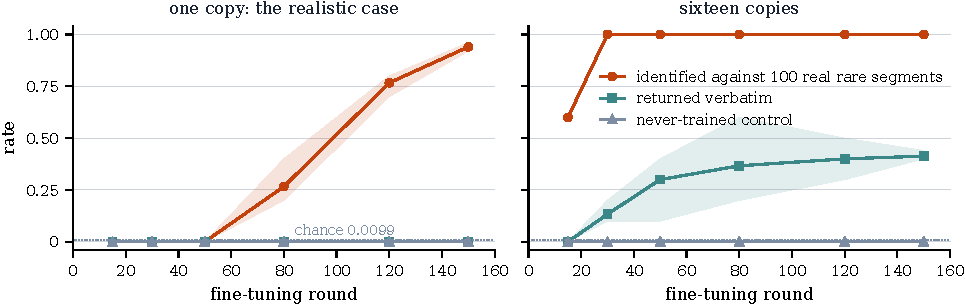
\includegraphics[width=\linewidth]{F6_ident.pdf}
\caption{DNABERT-2 fine-tuned on chromosome~22, three seeds; the band is the range over seeds.
\textbf{Left:} a haplotype planted once, which is the realistic case. Identification rises to 0.94
while verbatim recovery of the same records stays at zero at every checkpoint. \textbf{Right:} the
same records planted sixteen times, where verbatim recovery does move, so the zero on the left is
not a decoder unable to read this family at all. Never-trained controls are flat at zero in both
panels; the dotted line is chance, $0.0099$. Rounds 15--120 use 10 probes per tier and the last
round 50.}
\label{fig:ident}
\end{figure}

The control settles the obvious objection. Across 19 cells and 350 never-trained segments, not one
was ever ranked first. A probe loose enough to manufacture 0.94 out of nothing would have produced
false positives here, and it produced none.

\paragraph{Why this matters more than the reproduction numbers.}
Section~\ref{sec:leak} established that released models return records verbatim at a quality
practitioners would accept, which is the result that is easiest to act on. This one is the result
that is easiest to miss. A team following current practice plants canaries, measures extraction,
reads zero at single copy, and ships. The model they ship will, on being handed a candidate
haplotype, say whether that person was in the cohort: nine times in ten at the end of training, and
better than one in five from round~80 onward, which is well inside the range anyone would train to.
Both numbers therefore have to be reported. Either one on its own gives a misleading account of the
same weights.

\paragraph{A note on what is robust here.}
Identification is a ranking, and rankings are stable under the numerical noise that makes extraction
rates wobble (\S\ref{sec:measure}). Re-scoring a checkpoint months later on the same host after its
floating-point behaviour had changed reproduced every identification rate to the digit --- rank-1 at
$0.800$ before and after, held-out loss identical to four decimals --- while the extraction rate on
the same checkpoint moved by six points. The identification results in this table therefore do not
carry the uncertainty that \S\ref{sec:measure} attaches to the extraction results, and we quote them
without it.

% Privacy-first section 6: what decides whether a memorised record can be reached.
% Budget 1.5 pages including Table~\ref{tab:slots} and Figure~\ref{fig:slots}.
% Numbers: outputs/kcurve300 (window 300, k=1..6) replicated by outputs/kcurve (window 288);
% DNABERT family from outputs/dnabert_long/*_human_s0, re-measured 23 Oct. Notes 3.58(f), 3.59.
\section{What decides whether a leak can be reached}
\label{sec:slots}

Released models differ enormously in how much comes back out of them, and the obvious explanation
--- that some memorise more than others --- is wrong. This section shows that what varies is not how
much is stored but how many pieces have to be correct simultaneously to get it out, and that this is
set by the tokenizer.

\paragraph{The same knowledge, 92\% or 0\% out.}
Hold the backbone, the corpus, the optimiser and the schedule fixed, and vary only how the DNA is
split. Hiding 48 nucleotides then occupies $48/k$ token slots, and every slot has to be right at the
same time for the record to come back whole. Table~\ref{tab:slots} reads each run at matched held-out
loss rather than at a matched epoch, because the tokenizers converge at very different rates: at
round~30 every $k\ge3$ has saturated at 100\% and the comparison says nothing at all.

Two things in that table carry the claim. The extraction rate is monotone in the slot count with no
exception across six cut sizes, and the loss it costs to reach full extraction falls monotonically in
the same direction: 4.07\,\bits{} at 16 slots, 2.99 at 12, 2.63 at 9.6, 2.47 at 8, and never reached
at 24 or 48. A coarse tokenizer does not merely leak more. It leaks more cheaply, in the same
currency \S\ref{sec:leak} prices released checkpoints in.

\begin{table}[t]
\centering
\caption{From-scratch backbone, next-token objective, three seeds, uniform DNA, read at matched
held-out loss. \emph{Slots} is $48/k$, the number of token positions the hidden 48 nucleotides
occupy. \emph{Cost of 100\%} is the held-out loss at which extraction first reaches saturation.
Never-trained controls read $0.00$ in every tokenizer at every snapshot.}
\label{tab:slots}
\begin{tabular}{lcccccc}
\toprule
tokenizer & slots & @2.05 & @2.10 & @2.20 & @2.40 & cost of 100\% \\
\midrule
character        & 48  & ---  & ---  & ---  & ---  & never \\
\kmer{2}         & 24  & 0\%  & 0\%  & 0\%  & 0\%  & never \\
\kmer{3}         & 16  & 0\%  & 0\%  & 0\%  & 2\%  & 4.07 \\
\kmer{4}         & 12  & 0\%  & 0\%  & 2\%  & 12\% & 2.99 \\
\kmer{5}         & 9.6 & 0\%  & 2\%  & 24\% & 61\% & 2.63 \\
\kmer{6}         & 8   & 1\%  & 17\% & 67\% & 92\% & \textbf{2.47} \\
\bottomrule
\end{tabular}
\end{table}

The character rows are empty because the character model never reaches the comparison points: its
held-out loss stays between 2.00 and 2.04 for thirty epochs and its extraction rate stays at zero
throughout. It does not resist extraction after overfitting; it does not overfit far enough to be
asked.

\paragraph{The effect is not an artefact of the window.}
A reader may reasonably suspect a geometry that was chosen to make $48/k$ come out neatly. We
repeated the whole sweep at a second window length, 300\nt{} instead of 288, which changes the number
of host positions, the number of training tokens per window and the offsets every canary lands on.
Where the two windows share a tokenizer they agree closely: at matched loss $2.40$, \kmer{3} reads
2\% against 3\%, \kmer{4} 12\% against 11\%, \kmer{6} 92\% against 91\%, and the cost of full
extraction is 4.07/2.99/2.47 against 4.15/3.01/2.47. Two independent sets of eighteen and fifteen
runs, at different geometries, trace the same curve.

\paragraph{A prediction that could have falsified this, and did not.}
The slot account makes a claim about released models that is easy to check and awkward to explain
away if it fails. DNABERT ships four checkpoints differing only in $k$ \citep{ji2021dnabert}, which
looks like the ideal natural experiment --- but its $k$-mers \emph{overlap}, advancing one nucleotide
at a time, so the slot count stays near 48 whatever $k$ is. The slot account therefore predicts no
trend in that family at all, in contrast to the strong trend it predicts for non-overlapping
tokenizers. We recorded that prediction before measuring.

Fine-tuned on chromosome~22 with real haplotype canaries and read with a nucleotide-level decoder
matched to overlapping spans, the four checkpoints recover 2\%, 0\%, 4\% and 0\% of records planted
sixteen times, for $k=3,4,5,6$ respectively. There is no trend, as predicted.

\paragraph{The flat row is not ignorance.}
It would be a misreading to conclude that the overlapping family has memorised nothing. Asked for any
single nucleotide of a planted record with all the others supplied, those same four checkpoints
answer correctly 0.99--1.00 of the time, and the implied ceiling on whole-record recovery runs from
0.70 to 0.87. The records are in there, close to completely; 48 simultaneous slots is simply a wall
that our search cannot climb. This is the mechanism of \S\ref{sec:slots} appearing in a second place:
the same quantity that makes a 6-mer model leak at 2.47\,\bits{} makes an overlapping model look
clean while holding the same content.

Stated carefully, then, the finding is not that finer tokenisation memorises less. Both ends of
Table~\ref{tab:slots} learn a planted record to the same per-nucleotide accuracy. Coarser
tokenisation makes what was learned \emph{reachable}, and that is a different sentence to hand a
practitioner, with a different remedy attached.

% Privacy-first section 7: what a practitioner can do, and why the usual metric will not help.
% Budget 1.25 pages including Table~\ref{tab:blind} and Figure~\ref{fig:blind}.
% Early stopping: outputs/nt_{ckpt,seeds}/nt250m_mlm_ecoli_s*, ep3/ep15/ep50, one basis 19 Oct.
% Blind metric: outputs/nt_ckpt/nt250m_mlm_human_s0/utility_at_leak.json and bpe_human/*, 19-20 Oct.
\section{What a practitioner can do, and what will not warn them}
\label{sec:blind}

Two of the results above have an operational reading. Stopping where held-out loss stops improving
does prevent capture, but the margin is three hundredths of a bit, and the number practitioners
actually select on cannot resolve it.

\paragraph{At the optimum there is nothing to extract, because nothing is stored yet.}
It is worth distinguishing a record that is hidden from one that is absent. At the best saved
checkpoint of Nucleotide Transformer on \emph{E.~coli}, the leave-one-out probe, with every other
target nucleotide supplied and one masked, reads $0.01$, exactly the never-trained control, and the
planted
record's surprise is $2.128$ and $2.115$\,\bits{} against $2.110$ for a matched non-member. The
member is indistinguishable from a non-member on the model's own scale. No decoder can recover what
is not there, and our strongest decoder recovers 0\%.

Three hundredths of a bit later this is no longer true: across three seeds, 8\%, 8\% and 14\% of
records come back whole. Further out, at +0.44\,\bits, 66--76\%. The defence is real and the
transition is abrupt. Our own from-scratch backbone tolerates roughly ten times that drift before
leaking at all, so a study run only on a model one trains oneself reads more reassuringly than
released weights warrant. That is why this paper is built on released weights.

\paragraph{The number people select on moves by one per cent.}
Nobody chooses a genomic checkpoint by held-out loss. They choose by downstream task score.
Table~\ref{tab:blind} puts that score beside the leak at every checkpoint of the same runs.

\begin{table}[t]
\centering
\caption{Downstream task score measured at every checkpoint, beside the leak from the same weights.
GUE promoter classification, linear probe on frozen mean-pooled states, Matthews correlation on the
full held-out split. \emph{id} is single-copy identification as in \S\ref{sec:ident}.}
\label{tab:blind}
\begin{tabular}{llcccc}
\toprule
model & checkpoint & held-out \bits & MCC & 16-copy verbatim & 1-copy id \\
\midrule
NT 250M, chr22 & round 15 (best MCC) & 1.411 & \textbf{0.802} & \textbf{6\%}  & \textbf{0.04} \\
               & round 30            & 1.501 & 0.798          & 12\%          & 0.17 \\
               & round 50            & 1.632 & 0.780          & 18\%          & 0.35 \\
\midrule
DNABERT-2, chr22 & round 15 (best MCC) & 1.264 & 0.798--0.801 & 0\%   & 0.00 \\
                 & round 120           & 1.600 & 0.784--0.792 & 30--50\% & 0.70--0.80 \\
                 & final               & 1.729 & 0.782--0.787 & 40--44\% & 0.92--0.96 \\
\bottomrule
\end{tabular}
\end{table}

On DNABERT-2 the score declines across the run by 1.1--1.6 points of MCC in total, monotonically in
two seeds and with one reversal at round~50 in the third, while single-copy identification climbs
from nothing to 0.92--0.96 (Figure~\ref{fig:blind}). Selecting on that score
would pick round~15, which is also the safe checkpoint, so the metric is not misleading there. It
carries no information either: a practitioner watching it sees a flat line through the entire
interval in which the model learns to identify individuals.

On NT fine-tuned on chromosome~22 the situation is worse, because there is no clean checkpoint for
the metric to point at. The highest task score belongs to the earliest checkpoint saved, and that one
already reproduces 6\% of repeated records and identifies 4\% of single copies. Choosing the best
available model by downstream performance means choosing a model that is already leaking.

\begin{figure}[t]
\centering
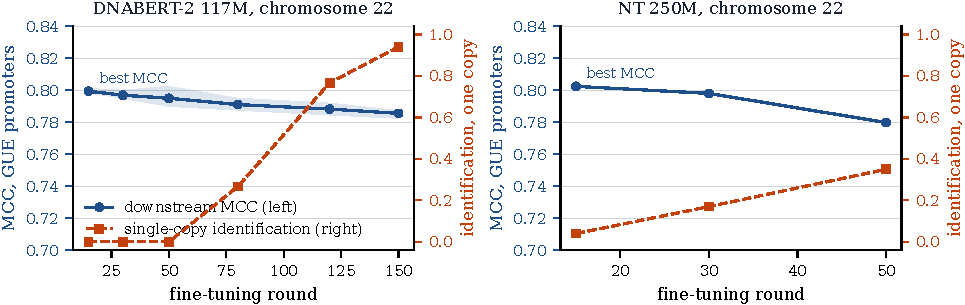
\includegraphics[width=\linewidth]{F7_blind.pdf}
\caption{Downstream score and leak, measured on the same weights at the same checkpoints.
\textbf{Left:} DNABERT-2 on chromosome~22, three seeds, band over seeds. The score falls by
1.1--1.6 points of MCC across a run in which single-copy identification goes from zero to 0.94.
\textbf{Right:} Nucleotide Transformer 250M on the same corpus, where the best downstream score is
the earliest checkpoint saved and that checkpoint already identifies 4\% of single copies. Linear
probe on frozen mean-pooled states, GUE promoter classification, full held-out split.}
\label{fig:blind}
\end{figure}


\paragraph{Recommendation.}
Three things follow, and we state them as the guidance we would give rather than as results.

\emph{Stop where held-out loss stops improving, and compute it.} It is the only quantity we measured
that moves before the leak does, and in a fine-tuning pipeline it is nearly free.

\emph{Do not treat downstream score as a safety signal.} Across six tasks and two organisms it never
moved more than one to two per cent while extraction went to saturation. It is evidence about
utility and nothing else.

\emph{Prefer a tokenizer with more slots, and measure what it costs you.} A model whose canary spans
24 or 48 token positions did not leak at any loss we drove it to, including losses far past
usefulness. That is the strongest protective effect we found. It is not free: fine-grained
tokenizers carry their own costs in sequence length and downstream accuracy, which are
task-dependent and which we did not measure across the board. We therefore offer the slot count as a
lever worth pricing rather than a setting we can recommend blind.

% Privacy-first section 8: limitations and discussion. Budget 0.75 page, no figure.
\section{Limitations and discussion}
\label{sec:discussion}

\paragraph{Cohort size is held fixed, and we do not know its effect.}
Every result here uses one fine-tuning corpus size. Scaling the number of individuals, or the amount
of sequence per individual, plausibly changes all of it: a planted record is a smaller fraction of
the gradient signal in a larger corpus, which argues for less memorisation, while a larger cohort
contains more rare haplotypes to confuse an identification probe, which argues for less
identification but also for a harder task. We tested neither direction. This is the first
experiment we would run next; it is cheap on the controlled backbone and expensive on released
weights.

\paragraph{The tokenisation result is scoped, and one released model sits outside the scope.}
Table~\ref{tab:slots} varies $k$ with the architecture, objective, optimiser and corpus fixed, which
is the only setting in which the axis is clean. It requires a model we train ourselves, because no
released family offers it. Across architectures the ordering does not survive: HyenaDNA, a released
single-nucleotide model at 14.2M parameters, almost exactly the size of our controlled backbone,
reaches 95\% verbatim extraction \citep{nguyen2023hyenadna}. That comparison varies architecture,
pretraining objective and objective-match simultaneously, so it does not contradict
\S\ref{sec:slots}; it bounds its generality. ``Finer tokenisation is safer'' is false as a general
claim and we do not make it.

\paragraph{The human arm is one chromosome.}
Canaries are drawn from chromosome~22 of a single cohort. Chromosome~21 appears only as pretraining
and replication. Nothing in the construction is chromosome-specific, but we have not shown that.

\paragraph{Our decoders are lower bounds, including where they read zero.}
We report whichever decoder is stronger per model, so every extraction figure understates what a
better attack could obtain. Two of our zeros are demonstrably decoder limits rather than model
properties: on DNABERT-2 the leave-one-out ceiling for single-copy records is 0.21--0.39 and on the
overlapping DNABERT family it is 0.70--0.87, while our searches return nothing in both cases. A reader
should treat those zeros as ``not reached by this attack'' and nothing more. From the same kind of
zero, the field currently draws the opposite inference.

\paragraph{Extraction rates carry more uncertainty than the probe count suggests.}
The re-masking decode is a discrete iteration and is sensitive to the model's last-bit arithmetic.
Re-running an identical cell after the host's floating-point behaviour changed moved its extraction
rate by six points, comparable to the binomial standard error on 50 probes (\S\ref{sec:measure}).
Identification does not share this sensitivity. Anyone reproducing these numbers should expect
agreement on identification to the digit and on extraction to within several points.

\paragraph{What we think this changes.}
The practical recommendation, which is to stop at the held-out optimum, is sound and nearly free,
but it rests on a quantity nobody in this field tracks, and the margin is three hundredths of a bit.
The second point concerns what a null result licenses. A team that plants canaries, measures extraction, reads
zero at single copy and ships has done what the literature currently asks, and has shipped a model
that will tell an adversary which of their participants it was trained on. Releasing fine-tuned
genomic weights should require reporting both numbers, measured with a decoder matched to the model's
own tokenizer, with a never-trained control scored in the same run. None of that is expensive, and
all of it is currently optional.


\paragraph{Acknowledgements.}
\TODO{funding and compute}

\bibliographystyle{plain}
\bibliography{refs}

\end{document}
